\chapter{Preliminares} % (fold)

\section{Definiciones}
\textbf{Criptografía.}
Es la ciencia que trata las escrituras ocultas, está comprendida por la Criptografía, el Criptoanálisis y la Esteganografía
La Criptografía es la ciencia que se encarga del estudio de técnicas para transformar la información a una forma que no pueda entenderse a simple vista; sin embargo, el objetivo de la Criptografía no es sólo mantener los datos secretos, sino también protegerlos contra modificación y comprobar la fuente de los mismos.

\textbf{Criptoanálisis}
Es la ciencia que se ocupa del análisis de un texto cifrado para obtener la información original sin conocimiento de la clave secreta, esto es, de forma ilícita rompiendo así los procedimientos de cifrado establecidos por la Criptografía, por lo que se dice que Criptoanálisis y Criptografía son ciencias complementarias pero contrarias.
El criptoanálisis es el arte de descifrar comunicaciones encriptadas sin conocer las llaves correctas

\subsection{Servicios criptográficos}
Los servicios de seguridad, son aquellos que garantizan en un sistema de información la adquisición, almacenamiento, procesamiento y transmisión de la información y para lograrlo se valen de uno o más mecanismos de seguridad.

\textbf{Confidencialidad}
Este servicio asegura que sólo las personas o procesos autorizados tengan acceso a la información. Con ello se busca que un agente no autorizado no pueda leer, copiar o modificar la información.
El servicio de confidencialidad se puede diferenciar en dos tipos:
\begin{itemize}
	\item Servicio de confidencialidad de contenido: se busca proteger el contenido de un recurso del sistema, para ello se cifra la información para que en caso ser interceptada por alguien no autorizado, no pueda ser descubierta. Este servicio puede proporcionar protección a todos los datos transmitidos por un usuario durante una conexión o puede proteger sólo parte de ellos por ejemplo sólo a los mensajes con información importante o incluso se pueden proteger sólo algunos campos de un determinado mensaje.
	\item Servicio de confidencialidad del mensaje: busca ocultar el flujo de un mensaje durante una conexión, para ello se cifra y se utiliza una técnica de envoltura con el objetivo de que si un atacante está realizando un análisis de tráfico, no pueda descubrir por ejemplo quien está enviando la información ni quien la recibe ni la frecuencia con la que se envían los mensajes.
\end{itemize}

\textbf{Autenticación}
Este servicio verifica la identidad de un agente que pretende acceder a la información. En una conexión entre dos entidades, el servicio verifica que las entidades sean quienes dicen ser, además de asegurar que un tercer individuo no pueda hacerse pasar por alguna de las entidades autorizadas y realizar una transmisión o recepción de datos.

\textbf{Integridad}
Este servicio asegura que el contenido de los datos no ha sido modificado y que la secuencia de los mismos se ha mantenido a lo largo de toda la transmisión, con ello se evita una réplica o un reordenamiento del mensaje por parte de un atacante.
Al igual que el servicio de confidencialidad, la integridad puede aplicarse a todos los datos transmitidos por un usuario durante una conexión, sólo a parte de ellos o sólo a algunos campos dentro del mensaje.
Cuando se tiene un ataque a la integridad de los datos, el sistema puede o no reportar dicha violación, por lo que se puede distinguir entre servicio de integridad con recuperación y servicio de integridad sin recuperación.
El servicio de integridad también se puede diferenciar entre servicio de integridad del contenido y servicio de integridad de la secuencia del mensaje
\begin{itemize}
	\item Servicio de integridad del contenido: proporciona pruebas de que el contenido no ha sido alterado o modificado.
	\item Servicio de integridad de la secuencia del mensaje: proporciona pruebas de que el orden de una secuencia de mensajes ha sido mantenida durante la transmisión.
\end{itemize}

\textbf{No repudio}
Este servicio evita que las entidades en una conexión nieguen haber transmitido o recibido un mensaje.
Existen varios tipos de este servicio y cada uno de ellos proporciona pruebas de haberse llevado a cabo:
\begin{itemize}
	\item No repudio de origen: con este servicio, el emisor de un mensaje no puede negar haber sido él quien transmitió dicho mensaje.
	\item No repudio de envío: comprueba que los datos fueron enviados.
	\item No repudio de presentación: protege contra cualquier intento falso de negar que los datos fueron presentados para el envío.
	\item No repudio de transporte: protege contra cualquier intento de negar que los datos fueron transportados.
	\item No repudio de recepción: con este servicio, el receptor de un mensaje no puede negar haber recibido un mensaje.
\end{itemize}


\section{Ataques a servicios criptográficos}
Un ataque es una violación a la seguridad de la información realizada por intrusos que tienen acceso físico al sistema sin ningún tipo de restricción, su objetivo es robar la información o hacer que ésta pierda valor relativo, o que disminuyan las posibilidades de su supervivencia a largo plazo.
%Un intruso puede obtener información como:
%\begin{itemize}
%	\item Bloques de direcciones IP
%	\item Localización de sistemas críticos (DNSs, WINS, DHCPs, Servidores de correo, etc.)
%	\item Puntos de acceso para números telefónicos y VPNs
%	\item Información personal de los trabajadores de la organización
%	\item Organizaciones asociadas, subsidiarias, etc.
%\end{itemize}
%Existen dos tipos de ataques que amenazan las comunicaciones secretas:
%\begin{itemize}
%	\item Pasivo: es aquel en el cual el intruso sólo busca obtener la información y al hacerlo no la modifica, por lo que es difícil percatarse de que se está siendo atacado.
%	\item Activo: el intruso además de obtener la información la modifica de tal modo que sirva a sus intereses y al ser modificada es más fácil percatarse de que se está siendo atacado.
%Los ataques activos se dividen en dos tipos: Ataques a los métodos de cifrado y Ataques a los protocolos criptográficos.
%\end{itemize}

%\textbf{Ataques a los Métodos de Cifrado}
%Este tipo de ataques se realizan con la intención de obtener la clave secreta para poder descifrar libremente cualquier criptograma, para ello se aprovechan las vulnerabilidades que pudiera tener el método de cifrado.

\textbf{Ataque sólo con texto cifrado}
Este caso es cuando el criptoanalista sólo conoce el criptograma y el algoritmo con que fue generado; con esta información pretende obtener el texto en claro.

\textbf{Ataque con texto original conocido}
En esta situación el criptoanalista conoce mensajes en claro seleccionados por él mismo y sus correspondientes criptogramas, así como el algoritmo con que éstos fueron generados; aquí el objetivo es conocer la clave secreta y poder descriptar libremente cualquier texto.

\textbf{Ataque con texto cifrado escogido}
El criptoanalista conoce el algoritmo de cifrado, así como un criptograma seleccionado por él mismo y su correspondiente texto en claro, su objetivo es obtener el mensaje en claro de todo criptograma que intercepte.

\textbf{Ataque con texto escogido}
En este caso el criptoanalista además de conocer el algoritmo de cifrado y el criptograma que quiere descriptar, también conoce el criptograma de un texto en claro que él elija y el mensaje en claro de un criptograma también elegido por él.

%\subsection{Ataques a los Protocolos Criptográficos}
%Este tipo de ataques no pretenden encontrar la clave secreta para poder conocer el mensaje en claro, sino que buscan obtener la información vulnerando los protocolos criptográficos, es decir, pretenden burlar la serie de pasos establecidos para alcanzar los objetivos de seguridad y que tienen que ser realizados por las entidades involucradas en cierta comunicación. Ejemplos de este tipo de ataques son los siguientes:

\textbf{Ataque con clave conocida}
El atacante conoce claves utilizadas en cifrados anteriores y con base en ellas intenta determinar nuevas claves.

%\subsection{SUPLANTACIÓN DE PERSONALIDAD}
%El atacante asume la identidad de uno de los agentes autorizados en la red, y de esta manera obtiene libremente y sin tropiezos todos los mensajes en claro.

%\subsection{COMPILACIÓN DE UN DICCIONARIO}
%Un diccionario es un archivo guardado en la memoria de la computadora que contiene contraseñas cifradas de los usuarios autorizados en el sistema. Si el método de cifrado con que se cifran las claves es público, el atacante puede generar claves aleatorias y después cifrarlas con el objeto de encontrar alguna contenida en el diccionario (previamente obtenido). Cuando una clave generada por el atacante coincide con una contenida en el diccionario, se ha encontrado una clave de acceso al sistema, mediante el usuario correspondiente a la clave encontrada.

%\subsection{BÚSQUEDA EXHAUSTIVA}
%Este ataque se lleva a cabo generando aleatoriamente todos los valores posibles de las claves de acceso y probándolas hasta que una de ellas sea una clave válida en el sistema.

\textbf{Ataque de hombre en medio}
El intruso se filtra en la línea de comunicación entre dos agentes autorizados en la red; obtiene la información de uno de ellos y se la envía al otro usuario una vez que la ha utilizado.

%\subsection{Ataques en criptoanálisis}
%Aunque para validar la robustez de un criptosistema normalmente se suponen todas las condiciones del peor caso, existen ataques más específicos, en los que no se cumplen todas estas condiciones. Cuando el método de ataque consiste simplemente en probar todas y cada una de las posibles claves del espacio de claves hasta encontrar la correcta, nos encontramos ante un ataque de fuerza bruta o ataque exhaustivo. Si el atacante conoce el algoritmo de cifrado y sólo tiene acceso al criptograma, se plantea un ataque sólo al criptograma; un caso más favorable para el criptoanalista se produce cuando el ataque cumple todas las condiciones del peor caso; en este caso, el criptoanálisis se denomina de texto en claro conocido. Si además el atacante puede cifrar una cantidad indeterminada de texto en claro al ataque se le denomina de texto en claro escogido; este es el caso habitual de los ataques contra el sistema de verificación de usuarios utilizado por Unix, donde un intruso consigue la tabla de contraseñas (generalmente /etc/passwd) y se limita a realizar cifrados de textos en claro de su elección y a comparar los resultados con las claves cifradas (a este ataque también se le llama de diccionario, debido a que el atacante suele utilizar un fichero `diccionario' con los textos en claro que va a utilizar). El caso más favorable para un analista se produce cuando puede obtener el texto en claro correspondiente a criptogramas de su elección; en este caso el ataque se denomina de texto cifrado escogido. 

%Cualquier algoritmo de cifrado, para ser considerado seguro, ha de soportar todos estos ataques y otros no citados; sin embargo, en la criptografía, como en cualquier aspecto de la seguridad, informática o no, no debemos olvidar un factor muy importante: las personas. El sistema más robusto caerá fácilmente si se tortura al emisor o al receptor hasta que desvelen el contenido del mensaje, o si se le ofrece a uno de ellos una gran cantidad de dinero; este tipo de ataques (sobornos, amenazas, extorsión, tortura...) se consideran siempre los más efectivos. 

\section{Criptografía Simétrica}
La criptografía simétrica utiliza la misma clave para cifrar y descifrar el mensaje de datos, es decir se basa en un secreto compartido~\cite{criptosimetrica}. \\ Características de la Criptografía simétrica: \begin{itemize}
	\item La clave es la misma para cifrar que para descifrar un mensaje, por lo que sólo el emisor y el receptor deben conocerla.
	\item Se basan en operaciones matemáticas sencillas, por ello son fácilmente implementados en hardware.
	\item Debido a su simplicidad matemática son capaces de cifrar grandes cantidades de datos en poco tiempo.
			       \end{itemize} ~\cite{sime} \\
Los algoritmos criptográficos simétricos tienen dos versiones: cifrador en bloque y cifrador en flujo. Una cifra es una palabra para describir un algoritmo de cifrado. El beneficio del uso de un algoritmo simétrico radica en el procesamiento rápido
para encriptar y desencriptar un alto volumen de datos. El cifrado simétrico es una eficaz táctica de almacenamiento de información
sensible en una base de datos, un registro o archivo ~\cite{sime} El cifrado simétrico puede ser representado con el siguiente diagrama ~\ref{fig:1-2-3}.

\begin{figure}[H]
\centering
	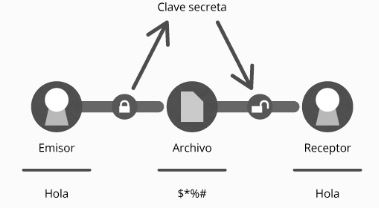
\includegraphics[width=10cm, height=5cm]{./images/Cripto_Simetrica.jpg}
	\caption{Diagrama Criptografía Simétrica}
	\label{fig:1-2-3}
\end{figure}
La sintaxis de un esquema de cifrado sim\'etrico, esta dada por la siguiente definic\'on.
\begin{definition} 
Un esquema de cifrado sim\'etrico est\'a conformado por una tripleta de algoritmos 
$\sf \Pi=(Gen, Enc, Dec)$, definidos como se describe a continuaci\'on:
\begin{itemize}
\item  El algoritmo generador de claves $\sf Gen$ selecciona una llave  $K$ al azar del conjunto de llaves $\cal K$, esto se denotar\'a como $K \rand {\cal K}$.
Esta clave $K$  ser\'a usada por los algoritmos  $\sf Enc$ y $\sf Dec$, esta clave la compartir\'an  emisor y receptor. 
\item El algoritmo de cifrado $\sf Enc$, toma como entrada un texto en claro  $M \in {\cal M}$ y una clave $K$ generada por  $\sf Gen$  y regresa un texto cifrado $C \in {\cal C}$.  Usualmente esto se denota como $C \leftarrow {\sf Enc}_K(M)$.
 \item El algoritmo de descifrado $\sf Dec$, toma como entrada un texto cifrado $C$ y una llave $K$ y regresa $M$. Esta operaci\'on se denota por  $M \leftarrow {\sf Dec}_K(C)$.
Para que cualquier algoritmo de cifrado sim\'etrico funcione correctamente, se debe garantizar que para
todas las llaves posibles en  $\cal K$ y todos los posibles mensajes $\cal M$, $$ {\sf Dec}_K({\sf Enc}_K(M)) = M.$$
\end{itemize}
\end{definition}

\section{Criptografía asimétrica}
La criptografía asimétrica es por definición aquella que utiliza dos claves diferentes para cada usuario, una para cifrar que se le llama clave pública y otra para descifrar que es la clave privada. Los algoritmos asimétricos son diferentes a los simétricos en un sentido muy importante ~\cite{sime}. Cuando se genera una clave simétrica, simplemente se escoge un número aleatorio de la longitud apropiada. Al generar claves asimétricas el proceso es más complejo. Los algoritmos asimétricos se llaman asimétricos porque en lugar de usar una sola clave para realizar la codificación y la decodificación, se utilizan dos claves diferentes: una para cifrar y otra para descifrar. Estas dos claves se encuentran asociadas matemáticamente, cuya característica fundamental es que una clave no puede descifrar lo que cifra. ~\cite{sime}.

\bigskip Características de la Criptografía simétrica: \begin{itemize}
	\item Se utiliza una clave para cifrar y otra para descifrar. El emisor emplea la clave pública del receptor para cifrar el mensaje, 	éste último lo descifra con su clave privada.
	\item Se basan en operaciones matemáticas complejas.
	\item Se ejecutan de 100 a 1000 veces más lento que los algoritmos simétricos.
\end{itemize} ~\cite{sime} \\ \\ 

 Los beneficios de la criptografía asimétrica son la solución a los problemas de la criptografía simétrica, pues las claves públicas pueden ser distribuidas con toda tranquilidad, no valen de nada sin las claves privadas. El cifrado asimétrico se le emplea muy frecuente para pasar con seguridad una clave privada, que posteriormente, será la que se utilice para cifrar y/o descifrar otra información. El cifrado asimétrico puede ser representado con el siguiente diagrama ~\ref{fig:1-2-4}.

\begin{figure}[H]
\centering
	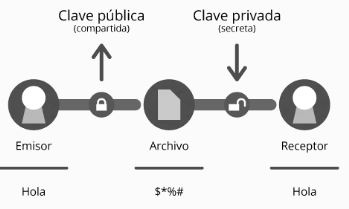
\includegraphics[width=10cm, height=5cm]{./images/Cripto_Asimetrica.jpg}
	\caption{Diagrama Criptografía Asimétrica}
	\label{fig:1-2-4}
\end{figure}

\section{Cifrado por bloques}
Los algoritmos de cifrado por bloques toman bloques de tamaño fijo del texto en claro y producen un bloque de tamaño fijo de texto cifrado, generalmente del mismo tamaño que la entrada. El tamaño del bloque debe ser lo suficientemente grande como para evitar ataques de texto cifrado. La asignación de bloques de entrada a bloques de salida debe ser uno a uno para hacer el proceso reversible y parecer aleatoria.\\ 
Para la asignación de bloques los algoritmos de cifrado simétrico realizan sustituciones y permutaciones en el texto en claro hasta obtener el texto cifrado.\\ 
La sustitución es el reemplazo de un valor de entrada por otro de los posibles valores de salida, en general, si usamos un tamaño de bloque k, el bloque de entrada puede ser sustituido por cualquiera de los 2k bloques posibles.
La permutación es un tipo especial de sustitución en el que los bits de un bloque de entrada son reordenados para producir el bloque cifrado, de este modo se preservan las estadísticas del bloque de entrada (el número de unos y ceros). \\ \\  Los algoritmos de cifrado por bloques iterativos funcionan aplicando en sucesivas rotaciones una transformación
(función de rotación) a un bloque de texto en claro. La misma función es aplicada a los datos usando una subclave
obtenida de la clave secreta proporcionada por el usuario. El número de rotaciones en un algoritmo de cifrado por
bloques iterativo depende del nivel de seguridad deseado.


La sustitución es el reemplazo de un bloque de $n$ bits por otro bloque de $n$ bits en un espacio de 
$2^{k}$~\cite{bloc}. Los cifradores por bloques mas usados son AES (Advanced Encryption Standard, por sus 
siglas en ingl\'es) y DES (Data Encryption Standard, por sus siglas en ingl\'es). \\ \\ Los cifradores por bloques pueden ser representados mediante el siguiente diagrama. ~\ref{fig:1-2-5}.

\begin{figure}[H]
\centering
	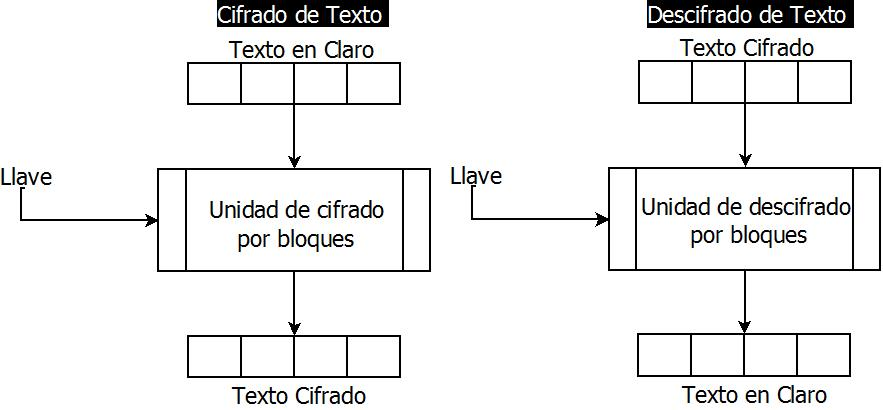
\includegraphics[width=10cm, height=5cm]{./images/CifradoBloques.jpeg}
	\caption{Diagrama Cifradores por Bloques}
	\label{fig:1-2-5}
\end{figure}



\section{Modos de operación}
Un modo de operación es una técnica para mejorar el efecto de un algoritmo criptográfico o adaptar el algoritmo para una aplicación, tal como aplicar un cifrador por bloques a una secuencia de bloques de datos o un flujo de datos. Los cuatro modos están destinados a cubrir virtualmente todas las aplicaciones posibles de cifrado para las cuales se podría usar un cifrador por bloques. A medida que han aparecido nuevas aplicaciones y requisitos, el NIST ha ampliado la lista de modos recomendados a cinco en la Publicación Especial 800-38A. Estos modos están diseñados para usarse con cualquier cifra simétrica de bloques, incluyendo DES triple y AES..\\\\


\textit{CBC}(Cipher-block chaining): La entrada al algoritmo de encriptación es el XOR de los siguientes 64 bits de texto plano y los 64 bits de cifrado anteriores.\\
\begin{itemize}
	\item La salida de uno de los bloques de cifrado se mete a otro bloque de cifrado junto con el siguiente bloque de mensaje.
	\item Toma como entradas un vector de inicialización (IV) y un bloque de mensaje (m).
	\item Durante el encriptado la salida del i - ésimo bloque depende del anterior i -1 bloques.
	\item La salida de cada uno de los bloques depende de todo lo anterior y esto lo hace mas seguro que ECB.
	\item  El descifrado de CBC es no secuencial.
\end{itemize}

\begin{figure}[h]
    \centering
    \begin{subfigure}[t]{0.5\textwidth}
        \centering
        \includegraphics[height=3in]{./images/CBC.png}
        \caption{Diagrama CBC Cifrado}
        \label{fig:1-3-1}
    \end{subfigure}
\end{figure}
\pagebreak

\textit{CFB}(Cipher Feedback): La entrada se procesa j bits a la vez. El texto cifrado precedente se utiliza como entrada al algoritmo de cifrado para producir la salida pseudoaleatoria, que se le aplica XOR con el texto sin formato para producir la siguiente unidad de texto cifrado.\\
\begin{itemize}
	\item Los bloques de cifrado también están encadenados pero la salida es muy diferente a los demás.
	\item Para cada bloque, el cifrado es producido haciendo XOR con el mensaje.
	\item Una ventaja de implementación es que no es necesaria la operación de descifrar no es necesario.
\end{itemize}

\begin{figure}[h]
    \centering
    \begin{subfigure}[t]{0.5\textwidth}
        \centering
        \includegraphics[height=3in]{./images/CFB.png}
        \caption{Diagrama CFB Cifrado}
        \label{fig:1-3-1}
    \end{subfigure}
\end{figure}
\pagebreak

\textit{OFB}(Output feedback): Similar a CFB, excepto que la entrada al algoritmo de cifrado es la salida DES anterior.\\
\begin{itemize}
	\item En OFB la salida del bloque de cifrado es alimentada de nuevo en la siguiente bloque de cifrado.
	\item El IV es cifrado varias veces para obtener una corriente de bytes aleatorios.
	\item Estas corrientes de bytes aleatorios se les hace XOR con el texto en plano para generar el texto cifrado.
\end{itemize}

\begin{figure}[h]
    \centering
    \begin{subfigure}[t]{0.5\textwidth}
        \centering
        \includegraphics[height=3in]{./images/OFB.png}
        \caption{Diagrama OFB Cifrado}
        \label{fig:1-3-1}
    \end{subfigure}
\end{figure}
\pagebreak

\textit{CTR}(Counter): Cada bloque de texto sin formato se le aplica XOR con un contador cifrado. El contador se incrementa para cada bloque subsiguiente.\\
\begin{itemize}
	\item CTR toma un vector de inicialización (IV) y en cada iteración el valor de IV se incrementa en 1 y queda cifrado.
	\item Para obtener el mensaje cifrado se hace una XOR con el IV y el bloque de mensaje.
	\item En términos de eficiencia CTR es mejor que CBC, OFB o CFB, ya que en este modo se pueden hacer las operaciones en paralelo ya que no dependen de algo para poder ser cifradas.
\end{itemize}

\begin{figure}[h]
    \centering
    \begin{subfigure}[t]{0.5\textwidth}
        \centering
        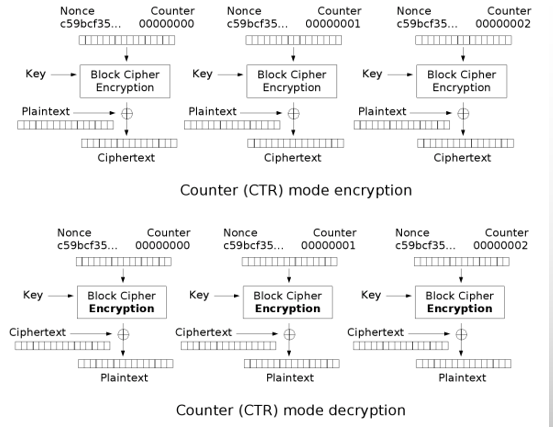
\includegraphics[height=3in]{./images/CTR.png}
        \caption{Diagrama CTR Cifrado}
        \label{fig:1-3-1}
    \end{subfigure}
\end{figure}


\pagebreak
\section{Funciones Hash}
A continuaci\'on se describir\'an las caracter\'isticas de las {\it funciones
hash}, tambi\'en conocidas como {\it funciones de resumen}. Las funciones hash basan
su definici\'on en funciones de un solo sentido  ({\it one-way functions}, en ingl\'es).
Una funci\'on de un s\'olo sentido es aquella que para un valor $x$, es 
muy f\'acil calcular $f(x)$, pero es muy dif\'icil hallar $f^{-1}(x)$. Es 
complicado en general, hallar funciones de \'este tipo y probar que lo 
son.
\begin{definition}
Una funci\'on hash, es una funci\'on de un s\'olo sentidocuya entrada $m$
 es un mensaje de longitud arbitraria
y la salida es una cadena binaria de longitud fija. Al resumen o hash de 
un mensaje $m$, se le denotar\'a como $h(m)$. Una funci\'on hash debe
tener las siguientes propiedades:
\begin{itemize}
\item Para cualquier mensaje $m$, debe ser posible calcular $h(m)$ 
eficientemente. 
\item Dado $h(m)$, debe ser computacionalmente dif\'icil, hallar un mensaje
$m'$, tal que $h(m)=h(m')$.
\item Debe ser computacionalmente dif\'icil, hallar dos mensajes $m$ y $m'$ 
tales que $h(m)=h(m')$.
\end{itemize}
\end{definition}
 
Entre las funciones hash que se usan para criptograf\'ia est\'an: MD2, MD4,
MD5, donde MD significa {\it Message Digest}, y el algoritmo est\'andar al momento de escribir \'estas notas es el {\it Secure Hash Algorithm} por sus siglas
en ingl\'es SHA.
  La MD5 fue dise\~nada por Ron Rivest, toma como entrada un mensaje de 
longitud arbitraria y proporciona como salida una cadena binaria de 128 bits.
El mensaje de entrada se procesa por bloques de 512 bits. 
  La SHA fue dise\~nada por en NIST y se estableci\'o como est\'andar
en 1993. Recibe como entrada un mensaje con longitud menor a $2^{64}$ bits y
como salida se obtiene una cadena binaria de 160 bits. Al igual que el
MD5, se procesa en bloques de 512 bits~\cite{modes}.
\pagebreak

\section{Cloud Computing (Cómputo Nube)}
El cómputo nube definido así por el NIST (National Institute of Standards and Technology), es un modelo para permitir un acceso a la red ubicuo, es decir, que se encuentra presente en todas partes al mismo tiempo y conveniente a un conjunto de recursos informáticos configurables (por ejemplo, redes, servidores, almacenamiento, aplicaciones y servicios) que se puede aprovisionar y liberar rápidamente con un esfuerzo mínimo de gestión o una interacción entre el proveedor de servicios.
Este modelo de cómputo nube se compone de 5 características esenciales, 3 modelos de servicio y 4  modelos de despliegue. 

\\ \\  \textbf{Características: }
\begin{itemize}
	\item \textbf {Auto-servicio bajo demanda} \\  Un consumidor puede proporcionar unilateralmente capacidades del tiempo del servidor y el almacenamiento en red, según se necesite automáticamente sin interacción con cada proveedor de servicios.
 	\item \textbf {Amplio acceso a la red} \\   Las capacidades están disponibles a través de la red y se accede a través de mecanismos que promueven el uso por plataformas de clienteheterogéneas finas o gruesas (por ejemplo, teléfonos móviles, tablets, computadoras portátiles y estaciones de trabajo)
	\item \textbf {Agrupación de recursos} \\ Los recursos informáticos del proveedor se agrupan para servir a múltiples consumidores utilizando un modelo de múlti- usuario, con diferentes recursos físicos y virtuales asignados dinámicamente y reasignados de acuerdo con la demanda del consumidor. Hay una sensación de independencia de ubicación en que el cliente generalmente no tiene control o conocimiento sobre la ubicación exacta de los recursos proporcionados, pero puede especificar la ubicación en un nivel superior de abstracción (por ejemplo, país, estado o centro de datos). Ejemplos de recursos incluyen almacenamiento, procesamiento, memoria y ancho de banda de la red.
	\item \textbf{Elasticidad rápida} \\ Las capacidades pueden ser suministradas elásticamente y liberadas, en algunos casos de forma automática, para escalar rápidamente hacia fuera y hacia adentro proporcional a la demanda. Para el consumidor, las capacidades disponibles para la provisión a menudo parecen ser ilimitadas y pueden ser apropiadas en cualquier cantidad en cualquier momento.
	\item \textbf{Servicio medido} \\ Los sistemas de cómputo nube controlan y optimizan automáticamente el uso de recursos aprovechando una capacidad de medición en algún nivel de abstracción apropiado al tipo de servicio (por ejemplo, almacenamiento, procesamiento, ancho de banda y cuentas de usuario activas). El uso de recursos puede ser monitoreado, controlado y reportado, proporcionando transparencia tanto para el proveedor como para el consumidor del servicio utilizado.
\end{itemize}

\\ \\ \textbf{Modelos de servicio: }

\begin{itemize}
	\item \textbf {Software como Servicio (SaaS).} \\ La capacidad proporcionada al consumidor es utilizar las aplicaciones del proveedor que se ejecutan en una infraestructura en la nube. Las aplicaciones son accesibles desde varios dispositivos cliente a través de una interfaz de cliente ligero, como un navegador web (por ejemplo, correo electrónico basado en web) o una interfaz de programa. El consumidor no gestiona ni controla la infraestructura oculta de la nube, incluyendo la red, los servidores, los sistemas operativos, el almacenamiento o incluso las capacidades de las aplicaciones individuales, con la posible excepción de las limitadas configuraciones específicas de la configuración de la aplicación.
	\item \textbf {Plataforma como Servicio (PaaS)} \\ La capacidad proporcionada al consumidor es desplegar en la infraestructura de la nube aplicaciones creadas por el consumidor, utilizando lenguajes de programación, bibliotecas, servicios y herramientas soportadas por el proveedor. El consumidor no gestiona ni controla la infraestructura oculta de la nube, incluyendo la red, los servidores , sistemas operativos o de almacenamiento, pero tiene control sobre las aplicaciones desplegadas y, posiblemente, configuración de configuración para el entorno de alojamiento de aplicaciones.
	\item \textbf {Infraestructura como Servicio (IaaS).} \\  La capacidad proporcionada al consumidor es proveer procesamiento, almacenamiento, redes y otros recursos de computación fundamentales donde el consumidor es capaz de desplegar y ejecutar software arbitrario, que puede incluir sistemas operativos y aplicaciones. El consumidor no gestiona ni controla la infraestructura subyacente de la nube, sino que tiene control sobre los sistemas operativos, el almacenamiento y las aplicaciones implementadas; Y posiblemente un control limitado de componentes de red selectos (por ejemplo, firewalls de host).
\end{itemize}



%Las funciones hash son usadas para construir una pequeña huella digital de la informaci\'on, si la informaci\'on es alterada tambi\'en la huella digital es alterada. Esta caracter\'istica hace que las funciones hash sean ampliamente usadas para verificar la integridad de datos.\\
%De manera formal, un funci\'on Hash es una Cuadrupla$(X,Y,K,H)$ donde:
%\begin{enumerate}
% \item $X$ es un conjunto de posibles mensajes.
% \item $Y$ es un conjunto finito de posibles resúmenes de mensajes o etiquetas de autenticación.
% \item $K$, el espacio de claves, es un conjunto finito de posibles claves.
% \item Para cada $k\quad \epsilon\quad K$, existe una función hash $h_k\quad \epsilon\quad H$. Parac ada $h_k: X \longrightarrow Y$.
% \cite{stinson}
%\end{enumerate}



